\chapter{Performance Analysis}\label{Ch:Analyze}

After tuning the neural network structure and action space, we began to analyze the performance of our models. In section \ref{perf}, we explain the metrics we used for evaluating the model. We establish the baseline results in section \ref{base}. We compare the models with dropout to the baseline in the rest of this chapter. Note that in section \ref{solve}, we present a model that solved the CarRacing game challenge.

\section{Performance Metrics} \label{perf}
We used two metrics to evaluate the performance of our models. First, we allowed the model to play 100 games and computed the average score. Although the racetracks in these games were random, we used the same 100 racetracks for all tests in order to compare performance between models. We also compute the standard deviation of these 100 scores. This performance metric is based on the OpenAI challenge to achieve an average score of 900 or more over 100 games. 

\begin{figure}[H]
\centering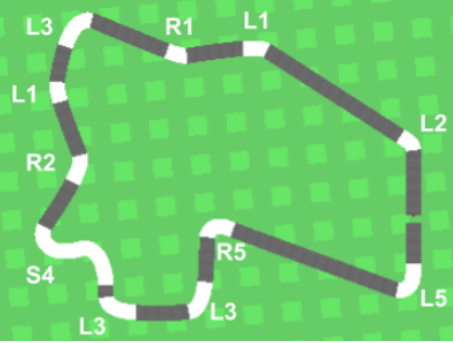
\includegraphics[scale=0.6,clip]
{Graphics/curve_characterization.png}
\caption[Curve Characterization]{An example of curve characterization}
\label{fig:curves}
\end{figure}

Second, we analyzed how the models performed on different curves in a racetrack. We developed a simple curve classification algorithm, which is demonstrated in Figure \ref{fig:curves}. Each curve is characterized as either as either a Left, Right, or S-shaped curve. An S-shaped curve is either a left turn followed by a right turn or a right turn followed by a left turn. Then, the steepness of the curve is ranked on a scale from 1 to 5, where 1 represents a very shallow curve and 5 represents a very steep curve. For example, L1 is a slight left curve and S4 is a fairly steep S-shaped curve. We compute the proportion of tiles that the agent visits for each class of curves. This performance metric is useful for understanding the strengths or weaknesses of a model as well as its ability to generalize to different curves.

\section{Baseline Results} \label{base}
We trained the algorithm on three environments and performed a baseline experiment. In the first environment, there was 1 predetermined racetrack that the agent interacts with during training.  In the second environment, there were 3 predetermined racetracks. In the third environment, the racetracks were generated randomly. The average score and standard deviation of testing these models over 100 random racetracks is shown in Table \ref{table:baseline_results}. 

\begin{table}[h]
\centering
\begin{tabular}{ m{4cm} | m{3cm}| m{3.5cm} } 
Model Environment & Average Score & Standard Deviation  \\
\hline 
1 Track & 849.99 & 78.72  \\
3 Track & 853.88 & 127.71  \\
Random Tracks & 854.83 & 107.14  \\
\end{tabular}
\caption{Baseline Performance over 100 random games}
\label{table:baseline_results}
\end{table}

The standard deviation of these test scores is fairly high because our current models are unable to perform well consistently. While testing these models, we observed that the algorithm struggled to generalize to different racetracks. For example, the model trained on a single fixed track catastrophically failed when it encountered a steep right curve during testing. We believe that this failure due to the fact that the model does not see any examples of steep right curves during training. This is an indicator that our algorithm is overfitting.

\section{Regularization with Dropout}
In order to prevent overfitting, we added dropout as a regularization technique to our neural network architecture by dropping out units at a rate of 30\% after the second convolutional layer of the neural network. We applied dropout to each of the three models tested in the baseline experiments in order to compare performance. The results of these experiments are shown in Table \ref{table:dropout}. 

\begin{table}[h]
\centering
\begin{tabular}{ m{4cm} | m{3cm}| m{3.5cm} } 
Model Environment & Average Score & Standard Deviation  \\
\hline 
1 Track & 894.38 & 24.5  \\
3 Tracks & 875.58 & 43.58 \\
Random Tracks & 887.39 & 24.65 \\
\end{tabular}
\caption{Performance for Dropout Rate 30\% over 100 random games}
\label{table:dropout}
\end{table}

When adding dropout to our neural network architecture, the average score over 100 games increased and standard deviation decreased in all three environments. The model achieved higher scores in the game more consistently. Hence, applying a dropout rate of 30\% improved the performance of our algorithm and came remarkably close to solving the OpenAI challenge of an average score of 900 over 100 random games.


\section{Curve Characterization}
We used the curve characterization method in order to determine whether applying dropout improved the ability of our algorithm to generalize to curves that were not seen during training. In particular, we analyzed the models that were trained on a single fixed track, because these models only saw a few curves durining training. Even though both models saw the same fixed track during training, the dropout model performed better on each class of steep curves. These results are demonstrated in Figure \ref{fig:dropout_curve}. These results indicate that using dropout allows the model to generalize better to curves it did not see during training. Thus, dropout has the potential to be an effective regularizer in deep reinforcement learning problems.

\begin{figure}[h!]
\centering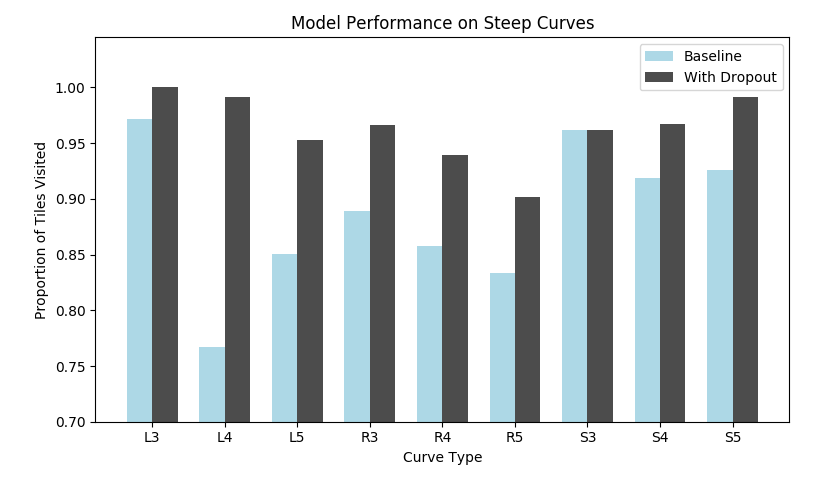
\includegraphics[scale=0.6,clip]
{Graphics/dropout_curve.png}
\caption[Curve Performance with Dropout]{Curve Performance with and without Dropout}
\label{fig:dropout_curve}
\end{figure}

\section{Solving Car Racing Game}\label{solve}
We then trained the neural network with dropping out units at a rate of 50\% to explore if higher dropout rate would improve the performance. The results of the experiments are shown in Table \ref{table:dropout_1}. 

\newpage
\begin{table}[h]
\centering
\begin{tabular}{ m{4cm} | m{3cm}| m{3.5cm} } 
Model Environment & Average Score & Standard Deviation \\ 
\hline 
3 Tracks & 906.67 & 23.6 \\
Random Tracks & 892.62 & 41.48 \\
\end{tabular}
\caption{Performance for Dropout Rate of 50\% over 100 random games}
\label{table:dropout_1}
\end{table}

Increasing the dropout rate from 30\% to 50\% increases the average score in all three environments. Using this method, we are able to achieve a score over 900 in the 3 Track environment, which successfully solves the OpenAI challenge.


\endinput

